%%
%% Author: Jordan Osborn
%% 01/01/2019
%%

% Preamble
\documentclass[11pt]{article}

% Packages
\usepackage{amsmath, mathrsfs}
\usepackage{titling}
\usepackage{hyperref}
\usepackage[sorting=none, backend=bibtex]{biblatex}
\usepackage{graphicx}
\usepackage{float}
\usepackage{enumitem}

\addbibresource{report.bib}

\title{A new video analysis algorithm for the study of crowd dynamics}
\author{Jordan Osborn (jo357) Supervisor: Professor Pietro Cicuta (pc245)}
% Document
\begin{document}
\begin{titlingpage}
    \maketitle
\end{titlingpage}


\clearpage
\title{A new video analysis algorithm for the study of crowd dynamics}
\author{Supervisor: Professor Pietro Cicuta (pc245)}
\maketitle
\section*{Abstract}

\clearpage
\tableofcontents
% TODO: 5000 Words 

\clearpage
\section{Introduction}
%TODO: Tuesday 16/04
In this project the technique of Differential Dynamic Microscopy will be applied to videos of crowd motion. This technique provides information about the dynamical behaviour of objects in a video without the use of image segmentation. DDM was first carried out in 2008, to analyse the dynamics of colloidal particles in Brownian motion \cite{ddm0}. A video of colloidal particles will be analysed and will act as a test case for the code developed in this project. Differential Dynamic Microscopy has primarily been used to analyse the motion of microscopic particles \cite{ddm1} \cite{ddm2}. This project was undertaken in order to determine the applicability of DDM to macroscopic motion i.e. crowd motion videos. A literature review will be carried out in section 2, but this will mainly be centred around the microscopic applications of DDM as prior literature is not available for the application of DDM to macroscopic motion. The code developed as a part of this project is intended to act as a reference for further development (e.g. for real time commercial crowd analysis) and so has been developed with execution speed as well as accuracy as a priority. Certain design decision were undertaken to achieve this. Further discussion about implementation will be carried out in section 3.
\\\\
In the figure below we see an outline of how DDM is carried out in the simple case of Brownian Motion. A detailed discussion of the theory behind DDM will occur in section 3. The information extractable from a DDM analysis is sensitive to the particular dynamics of the system for example for particles undergoing Brownian motion it is possible to extract the size of the diffusing particle\cite{ddm1}.


\begin{figure}[H]
\centering
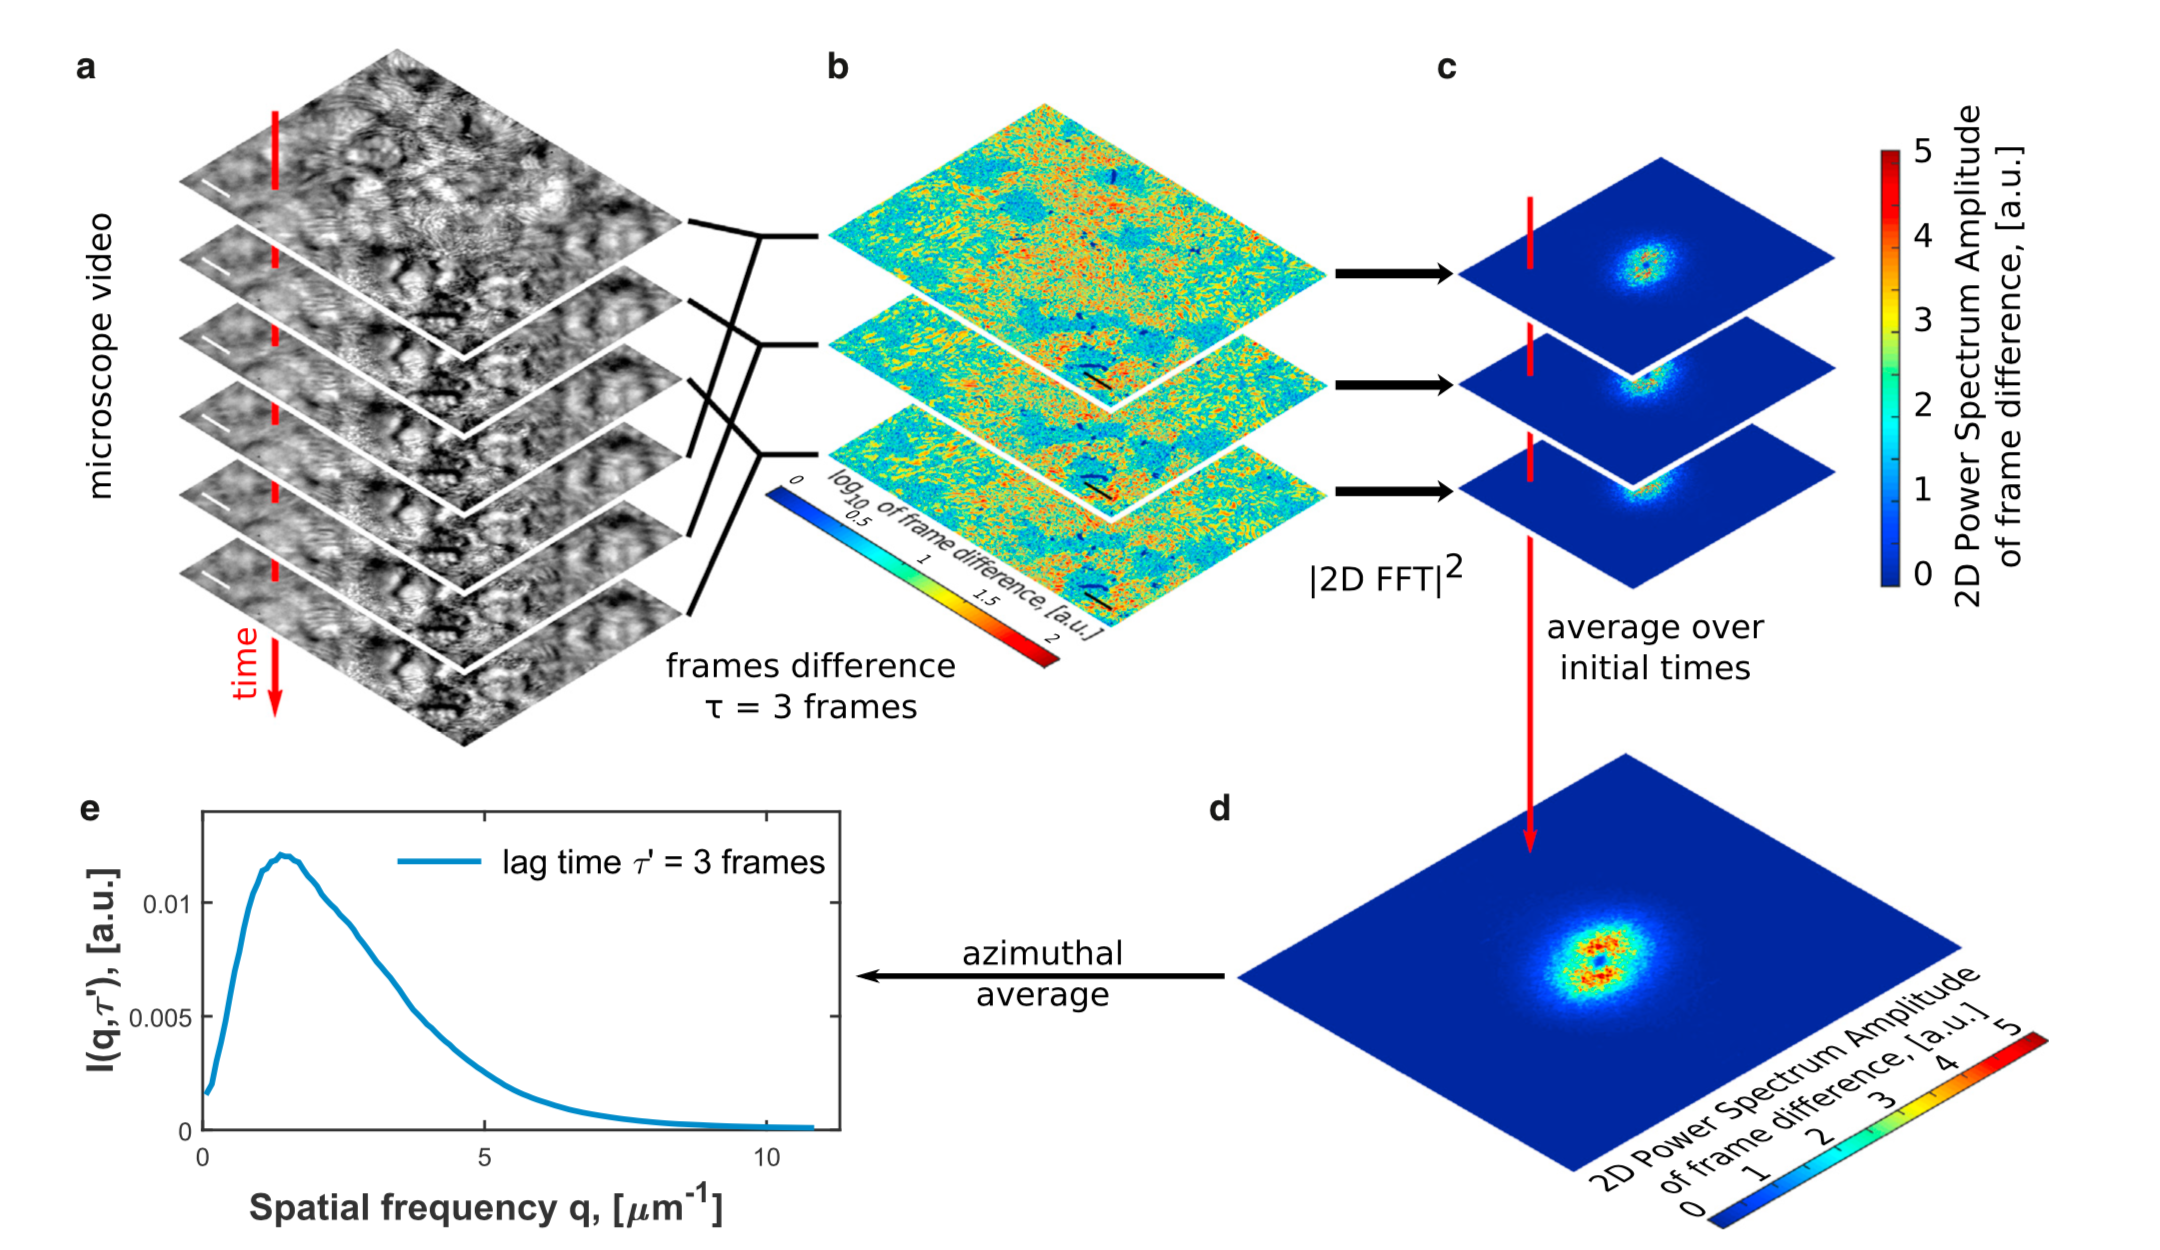
\includegraphics[height=5.5cm]{images/ddmpic.png}
\caption{Provides an overview of the DDM method as applied to the analysis of collective dynamics in ciliated cells.\cite{ddm2}}
\end{figure}

\begin{enumerate}[label=\alph*]
\item we take a video of the motion we wish to analyse and convert each frame into a 2D array of gray-scale pixel intensities.
\item for each starting frame in the video we take the difference between the pixel intensities of that frame and all lagging frames. $ \tau $ 
denotes the temporal separation of the two frames ( $ \tau = 3 $ frames,  is shown for various start times $ t_0 $). We denote each of these differences $ d(\underline{x}, t_0, \tau) $.
\item the 2D spatial Fourier transform of $ d(\underline{x}, t_0, \tau) $ is then taken for all combinations of $ t_0 $ and $ \tau $. Giving us d as a function of wave-vector instead of position. $ d(\underline{q}, t_0, \tau) $. We then take the the modulus squared of each Fourier transform giving us a power spectrum $I(\underline{q}, t_0, \tau) = |d(\underline{q}, t_0, \tau)|^2$.
\item because the system is stationary (power spectrum should be independent of $t_0$ and should only depend on $\tau$) we therefore take the average of the Fourier transforms over each $t_0$. This allows us to remove the dependence of $t_0$ from I and also reduce the effects of experimental uncertainty.
\item in the current case the system is also isotropic and so we can then take the azimuthal average of the 2D power spectrum. This means the power spectrum is now only a function of the modulus of the wave-vector q. $I(q, \tau)$
\item the expected functional form (for Brownian Motion) of this power spectrum has been proven to be $I(q, \tau) = A(q) \cdot (1 - e^{-\tau / \tau_c (q)}) + B(q)$ \cite{DLSPecora}. The physically interesting information is contained within $\tau_c$. $\tau_c$ for Brownian motion has been shown to equal $(D \cdot q^2)^{-1}$. Fitting the data (at each $\tau$) to this functional form and then extracting the value of $\tau_c$ as a function of q will yield the diffusion coefficient D. Plotting $log(\tau_c)$ against $log(q)$ should show a relationship of the form $y = -2\cdot x - log(D)$. The diffusion coefficient can then be used to find other pieces of information about the system including the size of the colloidal particles as there is a known relationship $D=\frac{k_B T}{6 \pi \eta R}$ between these two variables \cite{wynot_2002}.
\end{enumerate}
There are two primary types of DDM analysis. Single-scale DDM and Multi-scale DDM. Single-scale DDM performs DDM analysis on the entire image and so picks up a combination of the spatial and temporal scales of synchronisation \cite{ddm2}. Where as Multi-scale DDM performs DDM analysis on individual tilings of the image from a full-scale image down to the smallest tile size (determines the mini-mum wave-vector that can be compared across tiles)\cite{ddm2}. In this way spatial and temporal scales of synchronisation can be picked up separately. A more in-depth description of the two methods will take place in sections 3 and 4.  
\\\\
Each type of analysis will yield different pieces of dynamical information. Both methods will be run on a large database of approximately 400 videos\cite{crowdMotionDB}. The data will then be analysed, dynamical information will be extracted and then compared to that extractable by eye (for select videos). This analysis and discussion will take place in sections 5 and 6.
\\\\
DDM has the potential to be used to implement real-time analysis of crowd motion without the use of image segmentation, or the use of machine learning (expensive datasets and long training periods). Section 7 contains an in depth discussion about the future of DDM as applied to the analysis of crowd motion. The hope is that DDM might one day be used to help implement real-time crowd safety/monitoring systems in environments such as public transportation, stadiums, city centres etc.

\clearpage
\section{Literature Review}
%TODO: Friday 19/04

\clearpage
\section{Theory}
%TODO: Wednesday 17/04
% TODO: ddm in depth  activity, fitting dls scattering function, brownian motion, beat freq, crowd types, and fits, 


\clearpage
\section{Implementation}
%TODO: Thursday 18/04
rust\cite{arrayfire}

\clearpage
\section{Results}

\clearpage
\section{Discussion}

\clearpage
\section{Future}
%TODO: Saturday/Sunday 20-21/04/2019
\subsection{Comparisons}
\subsection{Advantages}
\subsection{Disadvantages}
\subsection{Applications}
\subsection{Further Development}

\clearpage
\section{Conclusion}


\clearpage
\section{References}
\printbibliography[heading=none]

\clearpage
\section{Appendices}
\subsection{Code}

\end{document}
